\documentclass[1p]{elsarticle_modified}
%\bibliographystyle{elsarticle-num}

%\usepackage[colorlinks]{hyperref}
%\usepackage{abbrmath_seonhwa} %\Abb, \Ascr, \Acal ,\Abf, \Afrak
\usepackage{amsfonts}
\usepackage{amssymb}
\usepackage{amsmath}
\usepackage{amsthm}
\usepackage{scalefnt}
\usepackage{amsbsy}
\usepackage{kotex}
\usepackage{caption}
\usepackage{subfig}
\usepackage{color}
\usepackage{graphicx}
\usepackage{xcolor} %% white, black, red, green, blue, cyan, magenta, yellow
\usepackage{float}
\usepackage{setspace}
\usepackage{hyperref}

\usepackage{tikz}
\usetikzlibrary{arrows}

\usepackage{multirow}
\usepackage{array} % fixed length table
\usepackage{hhline}

%%%%%%%%%%%%%%%%%%%%%
\makeatletter
\renewcommand*\env@matrix[1][\arraystretch]{%
	\edef\arraystretch{#1}%
	\hskip -\arraycolsep
	\let\@ifnextchar\new@ifnextchar
	\array{*\c@MaxMatrixCols c}}
\makeatother %https://tex.stackexchange.com/questions/14071/how-can-i-increase-the-line-spacing-in-a-matrix
%%%%%%%%%%%%%%%

\usepackage[normalem]{ulem}

\newcommand{\msout}[1]{\ifmmode\text{\sout{\ensuremath{#1}}}\else\sout{#1}\fi}
%SOURCE: \msout is \stkout macro in https://tex.stackexchange.com/questions/20609/strikeout-in-math-mode

\newcommand{\cancel}[1]{
	\ifmmode
	{\color{red}\msout{#1}}
	\else
	{\color{red}\sout{#1}}
	\fi
}

\newcommand{\add}[1]{
	{\color{blue}\uwave{#1}}
}

\newcommand{\replace}[2]{
	\ifmmode
	{\color{red}\msout{#1}}{\color{blue}\uwave{#2}}
	\else
	{\color{red}\sout{#1}}{\color{blue}\uwave{#2}}
	\fi
}

\newcommand{\Sol}{\mathcal{S}} %segment
\newcommand{\D}{D} %diagram
\newcommand{\A}{\mathcal{A}} %arc


%%%%%%%%%%%%%%%%%%%%%%%%%%%%%5 test

\def\sl{\operatorname{\textup{SL}}(2,\Cbb)}
\def\psl{\operatorname{\textup{PSL}}(2,\Cbb)}
\def\quan{\mkern 1mu \triangleright \mkern 1mu}

\theoremstyle{definition}
\newtheorem{thm}{Theorem}[section]
\newtheorem{prop}[thm]{Proposition}
\newtheorem{lem}[thm]{Lemma}
\newtheorem{ques}[thm]{Question}
\newtheorem{cor}[thm]{Corollary}
\newtheorem{defn}[thm]{Definition}
\newtheorem{exam}[thm]{Example}
\newtheorem{rmk}[thm]{Remark}
\newtheorem{alg}[thm]{Algorithm}

\newcommand{\I}{\sqrt{-1}}
\begin{document}

%\begin{frontmatter}
%
%\title{Boundary parabolic representations of knots up to 8 crossings}
%
%%% Group authors per affiliation:
%\author{Yunhi Cho} 
%\address{Department of Mathematics, University of Seoul, Seoul, Korea}
%\ead{yhcho@uos.ac.kr}
%
%
%\author{Seonhwa Kim} %\fnref{s_kim}}
%\address{Center for Geometry and Physics, Institute for Basic Science, Pohang, 37673, Korea}
%\ead{ryeona17@ibs.re.kr}
%
%\author{Hyuk Kim}
%\address{Department of Mathematical Sciences, Seoul National University, Seoul 08826, Korea}
%\ead{hyukkim@snu.ac.kr}
%
%\author{Seokbeom Yoon}
%\address{Department of Mathematical Sciences, Seoul National University, Seoul, 08826,  Korea}
%\ead{sbyoon15@snu.ac.kr}
%
%\begin{abstract}
%We find all boundary parabolic representation of knots up to 8 crossings.
%
%\end{abstract}
%\begin{keyword}
%    \MSC[2010] 57M25 
%\end{keyword}
%
%\end{frontmatter}

%\linenumbers
%\tableofcontents
%
\newcommand\colored[1]{\textcolor{white}{\rule[-0.35ex]{0.8em}{1.4ex}}\kern-0.8em\color{red} #1}%
%\newcommand\colored[1]{\textcolor{white}{ #1}\kern-2.17ex	\textcolor{white}{ #1}\kern-1.81ex	\textcolor{white}{ #1}\kern-2.15ex\color{red}#1	}

{\Large $\underline{12n_{0560}~(K12n_{0560})}$}

\setlength{\tabcolsep}{10pt}
\renewcommand{\arraystretch}{1.6}
\vspace{1cm}\begin{tabular}{m{100pt}>{\centering\arraybackslash}m{274pt}}
\multirow{5}{120pt}{
	\centering
	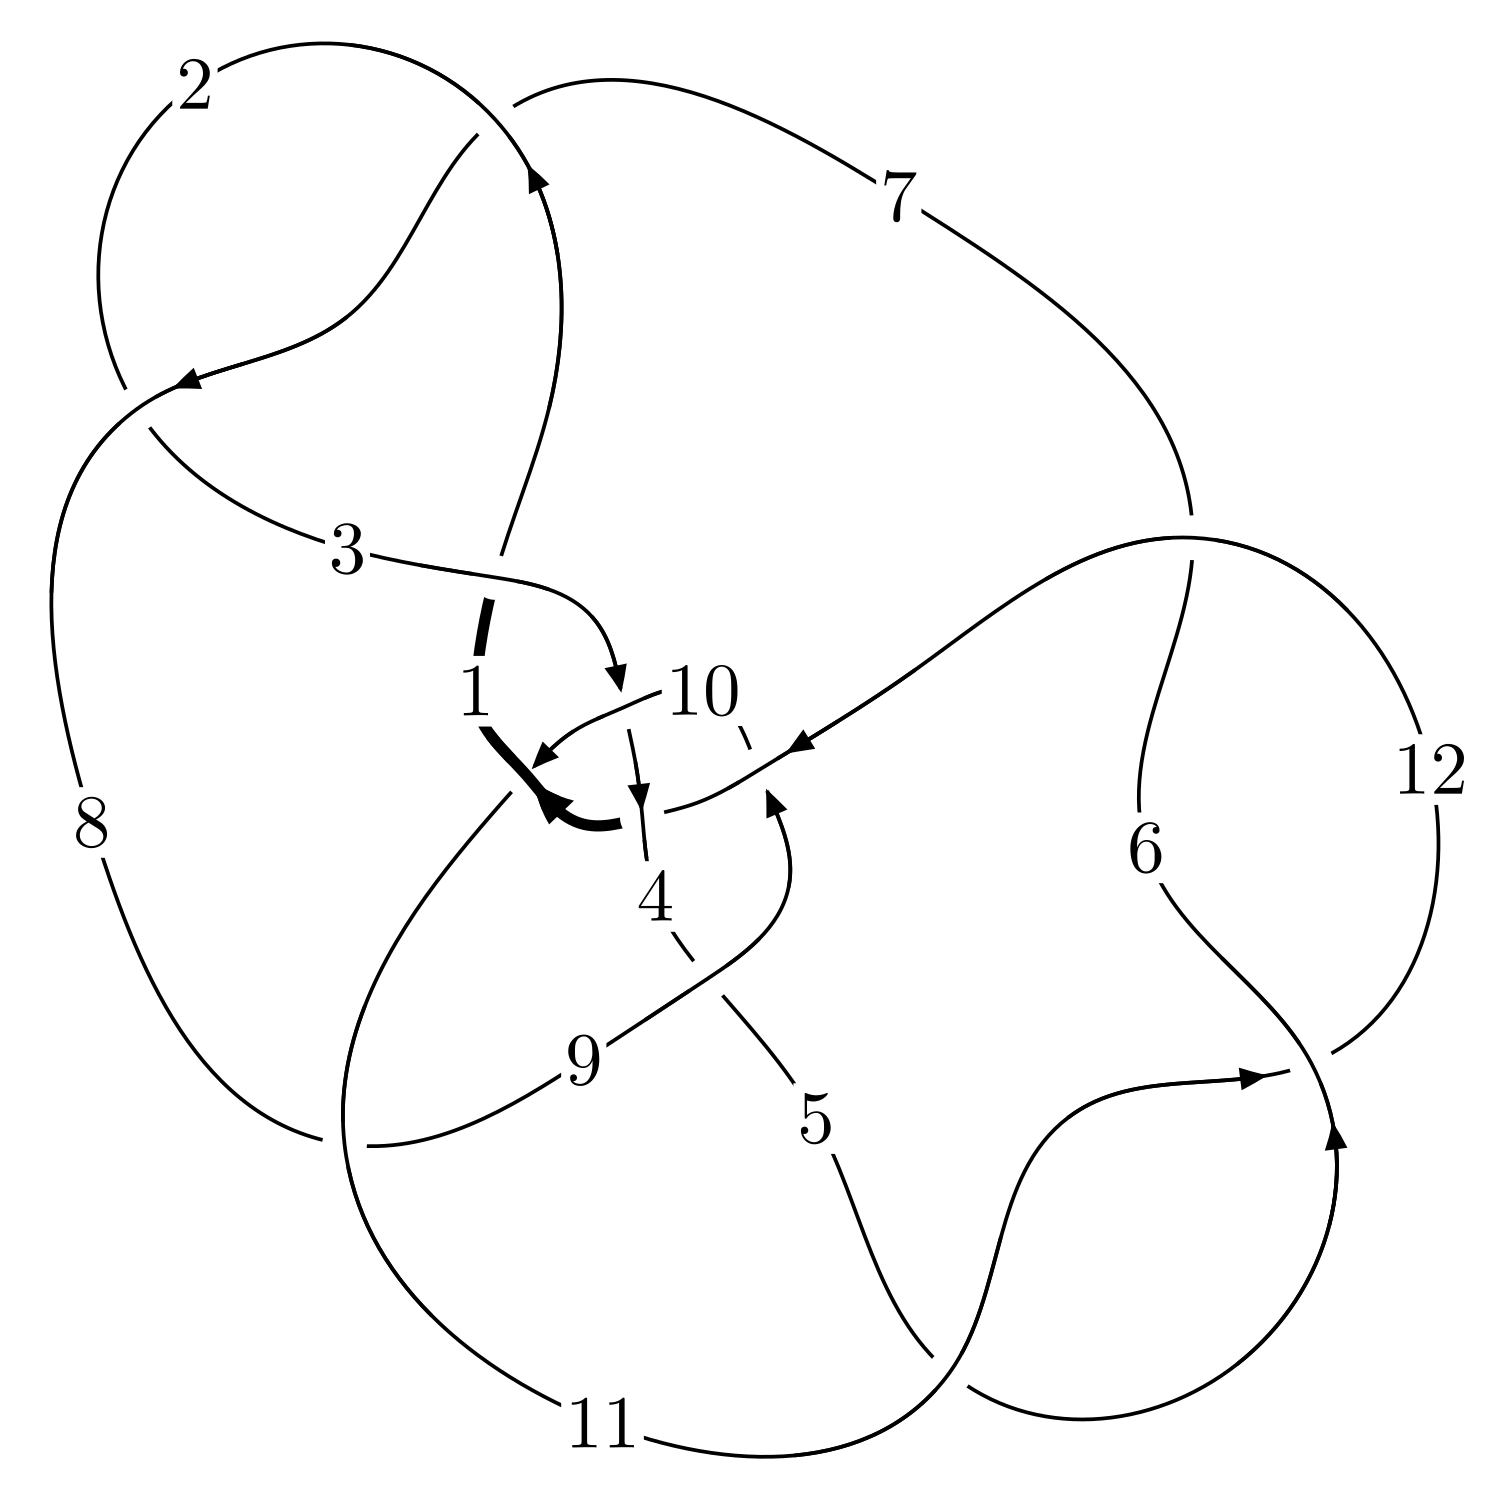
\includegraphics[width=112pt]{../../../GIT/diagram.site/Diagrams/png/2649_12n_0560.png}\\
\ \ \ A knot diagram\footnotemark}&
\allowdisplaybreaks
\textbf{Linearized knot diagam} \\
\cline{2-2}
 &
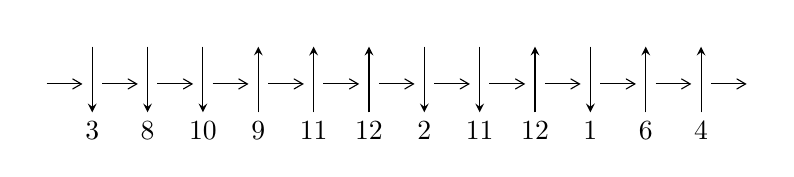
\begin{tikzpicture}[x=20pt, y=17pt]
	% nodes
	\node (C0) at (0, 0) {};
	\node (C1) at (1, 0) {};
	\node (C1U) at (1, +1) {};
	\node (C1D) at (1, -1) {3};

	\node (C2) at (2, 0) {};
	\node (C2U) at (2, +1) {};
	\node (C2D) at (2, -1) {8};

	\node (C3) at (3, 0) {};
	\node (C3U) at (3, +1) {};
	\node (C3D) at (3, -1) {10};

	\node (C4) at (4, 0) {};
	\node (C4U) at (4, +1) {};
	\node (C4D) at (4, -1) {9};

	\node (C5) at (5, 0) {};
	\node (C5U) at (5, +1) {};
	\node (C5D) at (5, -1) {11};

	\node (C6) at (6, 0) {};
	\node (C6U) at (6, +1) {};
	\node (C6D) at (6, -1) {12};

	\node (C7) at (7, 0) {};
	\node (C7U) at (7, +1) {};
	\node (C7D) at (7, -1) {2};

	\node (C8) at (8, 0) {};
	\node (C8U) at (8, +1) {};
	\node (C8D) at (8, -1) {11};

	\node (C9) at (9, 0) {};
	\node (C9U) at (9, +1) {};
	\node (C9D) at (9, -1) {12};

	\node (C10) at (10, 0) {};
	\node (C10U) at (10, +1) {};
	\node (C10D) at (10, -1) {1};

	\node (C11) at (11, 0) {};
	\node (C11U) at (11, +1) {};
	\node (C11D) at (11, -1) {6};

	\node (C12) at (12, 0) {};
	\node (C12U) at (12, +1) {};
	\node (C12D) at (12, -1) {4};
	\node (C13) at (13, 0) {};

	% arrows
	\draw[->,>={angle 60}]
	(C0) edge (C1) (C1) edge (C2) (C2) edge (C3) (C3) edge (C4) (C4) edge (C5) (C5) edge (C6) (C6) edge (C7) (C7) edge (C8) (C8) edge (C9) (C9) edge (C10) (C10) edge (C11) (C11) edge (C12) (C12) edge (C13) ;	\draw[->,>=stealth]
	(C1U) edge (C1D) (C2U) edge (C2D) (C3U) edge (C3D) (C4D) edge (C4U) (C5D) edge (C5U) (C6D) edge (C6U) (C7U) edge (C7D) (C8U) edge (C8D) (C9D) edge (C9U) (C10U) edge (C10D) (C11D) edge (C11U) (C12D) edge (C12U) ;
	\end{tikzpicture} \\
\hhline{~~} \\& 
\textbf{Solving Sequence} \\ \cline{2-2} 
 &
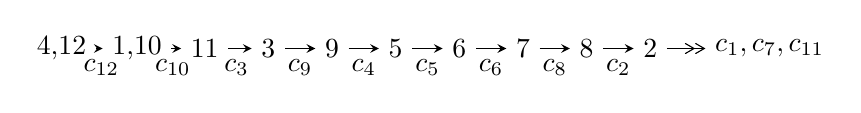
\begin{tikzpicture}[x=23pt, y=7pt]
	% node
	\node (A0) at (-1/8, 0) {4,12};
	\node (A1) at (17/16, 0) {1,10};
	\node (A2) at (17/8, 0) {11};
	\node (A3) at (25/8, 0) {3};
	\node (A4) at (33/8, 0) {9};
	\node (A5) at (41/8, 0) {5};
	\node (A6) at (49/8, 0) {6};
	\node (A7) at (57/8, 0) {7};
	\node (A8) at (65/8, 0) {8};
	\node (A9) at (73/8, 0) {2};
	\node (C1) at (1/2, -1) {$c_{12}$};
	\node (C2) at (13/8, -1) {$c_{10}$};
	\node (C3) at (21/8, -1) {$c_{3}$};
	\node (C4) at (29/8, -1) {$c_{9}$};
	\node (C5) at (37/8, -1) {$c_{4}$};
	\node (C6) at (45/8, -1) {$c_{5}$};
	\node (C7) at (53/8, -1) {$c_{6}$};
	\node (C8) at (61/8, -1) {$c_{8}$};
	\node (C9) at (69/8, -1) {$c_{2}$};
	\node (A10) at (11, 0) {$c_{1},c_{7},c_{11}$};

	% edge
	\draw[->,>=stealth]	
	(A0) edge (A1) (A1) edge (A2) (A2) edge (A3) (A3) edge (A4) (A4) edge (A5) (A5) edge (A6) (A6) edge (A7) (A7) edge (A8) (A8) edge (A9) ;
	\draw[->>,>={angle 60}]	
	(A9) edge (A10);
\end{tikzpicture} \\ 

\end{tabular} \\

\footnotetext{
The image of knot diagram is generated by the software ``\textbf{Draw programme}" developed by Andrew Bartholomew(\url{http://www.layer8.co.uk/maths/draw/index.htm\#Running-draw}), where we modified some parts for our purpose(\url{https://github.com/CATsTAILs/LinksPainter}).
}\phantom \\ \newline 
\centering \textbf{Ideals for irreducible components\footnotemark of $X_{\text{par}}$} 
 
\begin{align*}
I^u_{1}&=\langle 
1.42324\times10^{291} u^{90}-7.99634\times10^{291} u^{89}+\cdots+6.85609\times10^{290} b-1.64543\times10^{293},\\
\phantom{I^u_{1}}&\phantom{= \langle  }1.60031\times10^{293} u^{90}-1.04522\times10^{294} u^{89}+\cdots+3.22236\times10^{292} a+2.54763\times10^{294},\\
\phantom{I^u_{1}}&\phantom{= \langle  }u^{91}-7 u^{90}+\cdots+305 u-47\rangle \\
I^u_{2}&=\langle 
-2.64305\times10^{19} u^{24}+3.18164\times10^{19} u^{23}+\cdots+8.71996\times10^{19} b-3.13920\times10^{20},\\
\phantom{I^u_{2}}&\phantom{= \langle  }2.80082\times10^{20} u^{24}+7.55212\times10^{19} u^{23}+\cdots+8.71996\times10^{19} a+5.21556\times10^{20},\;u^{25}+2 u^{23}+\cdots+4 u-1\rangle \\
\\
\end{align*}
\raggedright * 2 irreducible components of $\dim_{\mathbb{C}}=0$, with total 116 representations.\\
\footnotetext{All coefficients of polynomials are rational numbers. But the coefficients are sometimes approximated in decimal forms when there is not enough margin.}
\newpage
\renewcommand{\arraystretch}{1}
\centering \section*{I. $I^u_{1}= \langle 1.42\times10^{291} u^{90}-8.00\times10^{291} u^{89}+\cdots+6.86\times10^{290} b-1.65\times10^{293},\;1.60\times10^{293} u^{90}-1.05\times10^{294} u^{89}+\cdots+3.22\times10^{292} a+2.55\times10^{294},\;u^{91}-7 u^{90}+\cdots+305 u-47 \rangle$}
\flushleft \textbf{(i) Arc colorings}\\
\begin{tabular}{m{7pt} m{180pt} m{7pt} m{180pt} }
\flushright $a_{4}=$&$\begin{pmatrix}0\\u\end{pmatrix}$ \\
\flushright $a_{12}=$&$\begin{pmatrix}1\\0\end{pmatrix}$ \\
\flushright $a_{1}=$&$\begin{pmatrix}1\\- u^2\end{pmatrix}$ \\
\flushright $a_{10}=$&$\begin{pmatrix}-4.96626 u^{90}+32.4364 u^{89}+\cdots+711.369 u-79.0609\\-2.07587 u^{90}+11.6631 u^{89}+\cdots-1257.99 u+239.995\end{pmatrix}$ \\
\flushright $a_{11}=$&$\begin{pmatrix}-4.98333 u^{90}+33.0713 u^{89}+\cdots+1492.91 u-209.668\\-2.27023 u^{90}+12.8918 u^{89}+\cdots-1099.99 u+215.772\end{pmatrix}$ \\
\flushright $a_{3}=$&$\begin{pmatrix}2.58074 u^{90}-20.1384 u^{89}+\cdots-790.887 u+148.913\\1.94318 u^{90}-13.7938 u^{89}+\cdots-338.479 u+33.8324\end{pmatrix}$ \\
\flushright $a_{9}=$&$\begin{pmatrix}-2.89039 u^{90}+20.7733 u^{89}+\cdots+1969.36 u-319.056\\-2.07587 u^{90}+11.6631 u^{89}+\cdots-1257.99 u+239.995\end{pmatrix}$ \\
\flushright $a_{5}=$&$\begin{pmatrix}1.50799 u^{90}-13.5634 u^{89}+\cdots-927.092 u+175.394\\-0.870427 u^{90}+7.21886 u^{89}+\cdots+476.684 u-60.3132\end{pmatrix}$ \\
\flushright $a_{6}=$&$\begin{pmatrix}-5.00106 u^{90}+32.5812 u^{89}+\cdots+1080.14 u-94.8173\\-0.980277 u^{90}+5.64049 u^{89}+\cdots-81.5790 u+47.6240\end{pmatrix}$ \\
\flushright $a_{7}=$&$\begin{pmatrix}-5.98134 u^{90}+38.2217 u^{89}+\cdots+998.557 u-47.1934\\-0.980277 u^{90}+5.64049 u^{89}+\cdots-81.5790 u+47.6240\end{pmatrix}$ \\
\flushright $a_{8}=$&$\begin{pmatrix}6.01042 u^{90}-36.3053 u^{89}+\cdots+462.327 u-156.674\\0.972663 u^{90}-4.59162 u^{89}+\cdots+973.368 u-177.396\end{pmatrix}$ \\
\flushright $a_{2}=$&$\begin{pmatrix}-0.270000 u^{90}+1.95357 u^{89}+\cdots+1656.96 u-236.764\\1.24299 u^{90}-9.26255 u^{89}+\cdots+183.479 u-30.9742\end{pmatrix}$\\&\end{tabular}
\flushleft \textbf{(ii) Obstruction class $= -1$}\\~\\
\flushleft \textbf{(iii) Cusp Shapes $= 0.0659084 u^{90}+0.108969 u^{89}+\cdots+1395.40 u-251.958$}\\~\\
\newpage\renewcommand{\arraystretch}{1}
\flushleft \textbf{(iv) u-Polynomials at the component}\newline \\
\begin{tabular}{m{50pt}|m{274pt}}
Crossings & \hspace{64pt}u-Polynomials at each crossing \\
\hline $$\begin{aligned}c_{1}\end{aligned}$$&$\begin{aligned}
&u^{91}+43 u^{90}+\cdots+22 u+1
\end{aligned}$\\
\hline $$\begin{aligned}c_{2},c_{7}\end{aligned}$$&$\begin{aligned}
&u^{91}+u^{90}+\cdots-11 u^2+1
\end{aligned}$\\
\hline $$\begin{aligned}c_{3}\end{aligned}$$&$\begin{aligned}
&u^{91}+2 u^{90}+\cdots-23 u+1
\end{aligned}$\\
\hline $$\begin{aligned}c_{4}\end{aligned}$$&$\begin{aligned}
&u^{91}+5 u^{90}+\cdots+95 u+82807
\end{aligned}$\\
\hline $$\begin{aligned}c_{5},c_{6},c_{11}\end{aligned}$$&$\begin{aligned}
&u^{91}-14 u^{89}+\cdots-6 u-11
\end{aligned}$\\
\hline $$\begin{aligned}c_{8}\end{aligned}$$&$\begin{aligned}
&u^{91}+11 u^{90}+\cdots-151800 u+12173
\end{aligned}$\\
\hline $$\begin{aligned}c_{9}\end{aligned}$$&$\begin{aligned}
&u^{91}-4 u^{90}+\cdots-12908 u+7912
\end{aligned}$\\
\hline $$\begin{aligned}c_{10}\end{aligned}$$&$\begin{aligned}
&u^{91}-3 u^{90}+\cdots+21 u-1
\end{aligned}$\\
\hline $$\begin{aligned}c_{12}\end{aligned}$$&$\begin{aligned}
&u^{91}+7 u^{90}+\cdots+305 u+47
\end{aligned}$\\
\hline
\end{tabular}\\~\\
\newpage\renewcommand{\arraystretch}{1}
\flushleft \textbf{(v) Riley Polynomials at the component}\newline \\
\begin{tabular}{m{50pt}|m{274pt}}
Crossings & \hspace{64pt}Riley Polynomials at each crossing \\
\hline $$\begin{aligned}c_{1}\end{aligned}$$&$\begin{aligned}
&y^{91}+17 y^{90}+\cdots-98 y-1
\end{aligned}$\\
\hline $$\begin{aligned}c_{2},c_{7}\end{aligned}$$&$\begin{aligned}
&y^{91}-43 y^{90}+\cdots+22 y-1
\end{aligned}$\\
\hline $$\begin{aligned}c_{3}\end{aligned}$$&$\begin{aligned}
&y^{91}+8 y^{90}+\cdots-29 y-1
\end{aligned}$\\
\hline $$\begin{aligned}c_{4}\end{aligned}$$&$\begin{aligned}
&y^{91}+77 y^{90}+\cdots-84473564657 y-6856999249
\end{aligned}$\\
\hline $$\begin{aligned}c_{5},c_{6},c_{11}\end{aligned}$$&$\begin{aligned}
&y^{91}-28 y^{90}+\cdots+10728 y-121
\end{aligned}$\\
\hline $$\begin{aligned}c_{8}\end{aligned}$$&$\begin{aligned}
&y^{91}-87 y^{90}+\cdots+8802996794 y-148181929
\end{aligned}$\\
\hline $$\begin{aligned}c_{9}\end{aligned}$$&$\begin{aligned}
&y^{91}+28 y^{90}+\cdots-2966219056 y-62599744
\end{aligned}$\\
\hline $$\begin{aligned}c_{10}\end{aligned}$$&$\begin{aligned}
&y^{91}+5 y^{90}+\cdots-85 y-1
\end{aligned}$\\
\hline $$\begin{aligned}c_{12}\end{aligned}$$&$\begin{aligned}
&y^{91}+17 y^{90}+\cdots-72509 y-2209
\end{aligned}$\\
\hline
\end{tabular}\\~\\
\newpage\flushleft \textbf{(vi) Complex Volumes and Cusp Shapes}
$$\begin{array}{c|c|c}  
\text{Solutions to }I^u_{1}& \I (\text{vol} + \sqrt{-1}CS) & \text{Cusp shape}\\
 \hline 
\begin{aligned}
u &= \phantom{-}1.01604\phantom{ +0.000000I} \\
a &= \phantom{-}1.19618\phantom{ +0.000000I} \\
b &= -0.619180\phantom{ +0.000000I}\end{aligned}
 & -2.35258\phantom{ +0.000000I} & \phantom{-0.000000 } 0 \\ \hline\begin{aligned}
u &= -0.535517 + 0.817566 I \\
a &= \phantom{-}0.40065 - 1.51679 I \\
b &= \phantom{-}0.79833 - 1.30743 I\end{aligned}
 & \phantom{-}2.27808 - 2.47811 I & \phantom{-0.000000 } 0 \\ \hline\begin{aligned}
u &= -0.535517 - 0.817566 I \\
a &= \phantom{-}0.40065 + 1.51679 I \\
b &= \phantom{-}0.79833 + 1.30743 I\end{aligned}
 & \phantom{-}2.27808 + 2.47811 I & \phantom{-0.000000 } 0 \\ \hline\begin{aligned}
u &= \phantom{-}0.502928 + 0.818348 I \\
a &= \phantom{-}0.26548 + 1.71837 I \\
b &= \phantom{-}0.71649 + 1.50318 I\end{aligned}
 & \phantom{-}1.57510 + 7.93270 I & \phantom{-0.000000 } 0 \\ \hline\begin{aligned}
u &= \phantom{-}0.502928 - 0.818348 I \\
a &= \phantom{-}0.26548 - 1.71837 I \\
b &= \phantom{-}0.71649 - 1.50318 I\end{aligned}
 & \phantom{-}1.57510 - 7.93270 I & \phantom{-0.000000 } 0 \\ \hline\begin{aligned}
u &= \phantom{-}0.511576 + 0.754182 I \\
a &= -0.282864 + 1.046630 I \\
b &= -0.15969 + 1.50698 I\end{aligned}
 & -3.58497 + 3.35574 I & \phantom{-0.000000 } 0 \\ \hline\begin{aligned}
u &= \phantom{-}0.511576 - 0.754182 I \\
a &= -0.282864 - 1.046630 I \\
b &= -0.15969 - 1.50698 I\end{aligned}
 & -3.58497 - 3.35574 I & \phantom{-0.000000 } 0 \\ \hline\begin{aligned}
u &= -0.340411 + 0.838886 I \\
a &= \phantom{-}2.01135 - 0.30444 I \\
b &= \phantom{-}0.224821 + 0.577269 I\end{aligned}
 & -5.14562 + 4.77451 I & \phantom{-0.000000 } 0 \\ \hline\begin{aligned}
u &= -0.340411 - 0.838886 I \\
a &= \phantom{-}2.01135 + 0.30444 I \\
b &= \phantom{-}0.224821 - 0.577269 I\end{aligned}
 & -5.14562 - 4.77451 I & \phantom{-0.000000 } 0 \\ \hline\begin{aligned}
u &= \phantom{-}0.402058 + 1.018890 I \\
a &= \phantom{-}0.309845 + 0.736789 I \\
b &= \phantom{-}0.920317 + 0.286799 I\end{aligned}
 & \phantom{-}1.85645 + 0.03554 I & \phantom{-0.000000 } 0\\
 \hline 
 \end{array}$$\newpage$$\begin{array}{c|c|c}  
\text{Solutions to }I^u_{1}& \I (\text{vol} + \sqrt{-1}CS) & \text{Cusp shape}\\
 \hline 
\begin{aligned}
u &= \phantom{-}0.402058 - 1.018890 I \\
a &= \phantom{-}0.309845 - 0.736789 I \\
b &= \phantom{-}0.920317 - 0.286799 I\end{aligned}
 & \phantom{-}1.85645 - 0.03554 I & \phantom{-0.000000 } 0 \\ \hline\begin{aligned}
u &= \phantom{-}0.285864 + 0.847239 I \\
a &= \phantom{-}1.201830 + 0.295601 I \\
b &= -0.237159 - 0.435090 I\end{aligned}
 & -3.55210 - 0.95036 I & \phantom{-0.000000 } 0 \\ \hline\begin{aligned}
u &= \phantom{-}0.285864 - 0.847239 I \\
a &= \phantom{-}1.201830 - 0.295601 I \\
b &= -0.237159 + 0.435090 I\end{aligned}
 & -3.55210 + 0.95036 I & \phantom{-0.000000 } 0 \\ \hline\begin{aligned}
u &= -0.713254 + 0.852005 I \\
a &= \phantom{-}0.590412 - 0.913948 I \\
b &= \phantom{-}1.40202 - 0.39992 I\end{aligned}
 & \phantom{-}2.06775 - 4.11651 I & \phantom{-0.000000 } 0 \\ \hline\begin{aligned}
u &= -0.713254 - 0.852005 I \\
a &= \phantom{-}0.590412 + 0.913948 I \\
b &= \phantom{-}1.40202 + 0.39992 I\end{aligned}
 & \phantom{-}2.06775 + 4.11651 I & \phantom{-0.000000 } 0 \\ \hline\begin{aligned}
u &= -0.375828 + 0.777228 I \\
a &= \phantom{-}2.13286 + 0.69059 I \\
b &= \phantom{-}0.149648 + 1.035570 I\end{aligned}
 & -5.60570 - 1.85793 I & \phantom{-0.000000 } 0 \\ \hline\begin{aligned}
u &= -0.375828 - 0.777228 I \\
a &= \phantom{-}2.13286 - 0.69059 I \\
b &= \phantom{-}0.149648 - 1.035570 I\end{aligned}
 & -5.60570 + 1.85793 I & \phantom{-0.000000 } 0 \\ \hline\begin{aligned}
u &= \phantom{-}0.058258 + 1.148570 I \\
a &= -0.157026 + 0.120099 I \\
b &= -1.033890 - 0.104076 I\end{aligned}
 & -0.18986 - 2.74164 I & \phantom{-0.000000 } 0 \\ \hline\begin{aligned}
u &= \phantom{-}0.058258 - 1.148570 I \\
a &= -0.157026 - 0.120099 I \\
b &= -1.033890 + 0.104076 I\end{aligned}
 & -0.18986 + 2.74164 I & \phantom{-0.000000 } 0 \\ \hline\begin{aligned}
u &= -0.741814 + 0.880371 I \\
a &= \phantom{-}0.571332 - 1.268100 I \\
b &= \phantom{-}1.232440 - 0.542664 I\end{aligned}
 & \phantom{-}1.99911 - 1.44766 I & \phantom{-0.000000 } 0\\
 \hline 
 \end{array}$$\newpage$$\begin{array}{c|c|c}  
\text{Solutions to }I^u_{1}& \I (\text{vol} + \sqrt{-1}CS) & \text{Cusp shape}\\
 \hline 
\begin{aligned}
u &= -0.741814 - 0.880371 I \\
a &= \phantom{-}0.571332 + 1.268100 I \\
b &= \phantom{-}1.232440 + 0.542664 I\end{aligned}
 & \phantom{-}1.99911 + 1.44766 I & \phantom{-0.000000 } 0 \\ \hline\begin{aligned}
u &= -0.504843 + 0.650504 I \\
a &= -0.093611 - 1.221940 I \\
b &= \phantom{-}1.16969 - 2.24380 I\end{aligned}
 & -5.05641 - 1.58259 I & \phantom{-0.000000 } 0 \\ \hline\begin{aligned}
u &= -0.504843 - 0.650504 I \\
a &= -0.093611 + 1.221940 I \\
b &= \phantom{-}1.16969 + 2.24380 I\end{aligned}
 & -5.05641 + 1.58259 I & \phantom{-0.000000 } 0 \\ \hline\begin{aligned}
u &= \phantom{-}0.414171 + 0.694826 I \\
a &= -0.85543 + 1.18748 I \\
b &= \phantom{-}0.63014 + 1.40371 I\end{aligned}
 & -3.09163 + 4.24015 I & \phantom{-0.000000 } 0 \\ \hline\begin{aligned}
u &= \phantom{-}0.414171 - 0.694826 I \\
a &= -0.85543 - 1.18748 I \\
b &= \phantom{-}0.63014 - 1.40371 I\end{aligned}
 & -3.09163 - 4.24015 I & \phantom{-0.000000 } 0 \\ \hline\begin{aligned}
u &= \phantom{-}0.460264 + 1.102830 I \\
a &= -0.375405 + 0.085886 I \\
b &= -1.151740 + 0.417119 I\end{aligned}
 & -0.85952 - 3.02137 I & \phantom{-0.000000 } 0 \\ \hline\begin{aligned}
u &= \phantom{-}0.460264 - 1.102830 I \\
a &= -0.375405 - 0.085886 I \\
b &= -1.151740 - 0.417119 I\end{aligned}
 & -0.85952 + 3.02137 I & \phantom{-0.000000 } 0 \\ \hline\begin{aligned}
u &= \phantom{-}0.742276 + 0.943517 I \\
a &= \phantom{-}0.31758 + 1.38675 I \\
b &= \phantom{-}1.227720 + 0.697519 I\end{aligned}
 & \phantom{-}1.14861 + 5.13293 I & \phantom{-0.000000 } 0 \\ \hline\begin{aligned}
u &= \phantom{-}0.742276 - 0.943517 I \\
a &= \phantom{-}0.31758 - 1.38675 I \\
b &= \phantom{-}1.227720 - 0.697519 I\end{aligned}
 & \phantom{-}1.14861 - 5.13293 I & \phantom{-0.000000 } 0 \\ \hline\begin{aligned}
u &= \phantom{-}0.284021 + 0.743601 I \\
a &= \phantom{-}1.24425 - 0.68339 I \\
b &= -0.230665 - 1.105310 I\end{aligned}
 & -3.42068 - 1.44050 I & \phantom{-0.000000 } 0\\
 \hline 
 \end{array}$$\newpage$$\begin{array}{c|c|c}  
\text{Solutions to }I^u_{1}& \I (\text{vol} + \sqrt{-1}CS) & \text{Cusp shape}\\
 \hline 
\begin{aligned}
u &= \phantom{-}0.284021 - 0.743601 I \\
a &= \phantom{-}1.24425 + 0.68339 I \\
b &= -0.230665 + 1.105310 I\end{aligned}
 & -3.42068 + 1.44050 I & \phantom{-0.000000 } 0 \\ \hline\begin{aligned}
u &= \phantom{-}0.910189 + 0.791577 I \\
a &= -0.01089 - 1.43365 I \\
b &= -1.095740 - 0.429637 I\end{aligned}
 & \phantom{-}0.52246 + 9.04938 I & \phantom{-0.000000 } 0 \\ \hline\begin{aligned}
u &= \phantom{-}0.910189 - 0.791577 I \\
a &= -0.01089 + 1.43365 I \\
b &= -1.095740 + 0.429637 I\end{aligned}
 & \phantom{-}0.52246 - 9.04938 I & \phantom{-0.000000 } 0 \\ \hline\begin{aligned}
u &= -0.302014 + 0.713600 I \\
a &= -2.26078 - 1.63663 I \\
b &= \phantom{-}0.159232 - 1.216630 I\end{aligned}
 & -5.43065 - 8.18174 I & \phantom{-0.000000 } 0 \\ \hline\begin{aligned}
u &= -0.302014 - 0.713600 I \\
a &= -2.26078 + 1.63663 I \\
b &= \phantom{-}0.159232 + 1.216630 I\end{aligned}
 & -5.43065 + 8.18174 I & \phantom{-0.000000 } 0 \\ \hline\begin{aligned}
u &= -0.480089 + 0.602783 I \\
a &= \phantom{-}0.353743 - 0.681474 I \\
b &= \phantom{-}2.04861 - 1.58222 I\end{aligned}
 & -4.22204 - 8.04480 I & \phantom{-0.000000 } 0 \\ \hline\begin{aligned}
u &= -0.480089 - 0.602783 I \\
a &= \phantom{-}0.353743 + 0.681474 I \\
b &= \phantom{-}2.04861 + 1.58222 I\end{aligned}
 & -4.22204 + 8.04480 I & \phantom{-0.000000 } 0 \\ \hline\begin{aligned}
u &= -0.497589 + 0.584067 I \\
a &= \phantom{-}0.377588 - 0.738280 I \\
b &= \phantom{-}0.097090 - 0.481940 I\end{aligned}
 & \phantom{-}0.092786 - 1.282950 I & \phantom{-0.000000 } 0 \\ \hline\begin{aligned}
u &= -0.497589 - 0.584067 I \\
a &= \phantom{-}0.377588 + 0.738280 I \\
b &= \phantom{-}0.097090 + 0.481940 I\end{aligned}
 & \phantom{-}0.092786 + 1.282950 I & \phantom{-0.000000 } 0 \\ \hline\begin{aligned}
u &= -0.673714 + 0.358408 I \\
a &= \phantom{-}0.06705 + 1.69725 I \\
b &= -0.034930 + 0.383069 I\end{aligned}
 & \phantom{-}3.79905 - 0.34651 I & \phantom{-0.000000 } 0\\
 \hline 
 \end{array}$$\newpage$$\begin{array}{c|c|c}  
\text{Solutions to }I^u_{1}& \I (\text{vol} + \sqrt{-1}CS) & \text{Cusp shape}\\
 \hline 
\begin{aligned}
u &= -0.673714 - 0.358408 I \\
a &= \phantom{-}0.06705 - 1.69725 I \\
b &= -0.034930 - 0.383069 I\end{aligned}
 & \phantom{-}3.79905 + 0.34651 I & \phantom{-0.000000 } 0 \\ \hline\begin{aligned}
u &= \phantom{-}0.446976 + 0.607186 I \\
a &= -0.141520 + 0.286604 I \\
b &= \phantom{-}1.50527 + 1.04718 I\end{aligned}
 & -2.59552 + 3.93278 I & \phantom{-0.000000 } 0 \\ \hline\begin{aligned}
u &= \phantom{-}0.446976 - 0.607186 I \\
a &= -0.141520 - 0.286604 I \\
b &= \phantom{-}1.50527 - 1.04718 I\end{aligned}
 & -2.59552 - 3.93278 I & \phantom{-0.000000 } 0 \\ \hline\begin{aligned}
u &= \phantom{-}0.363853 + 0.660110 I \\
a &= -1.45967 + 0.78808 I \\
b &= \phantom{-}0.537801 + 1.081090 I\end{aligned}
 & -3.13954 + 4.13473 I & \phantom{-0.000000 } 0 \\ \hline\begin{aligned}
u &= \phantom{-}0.363853 - 0.660110 I \\
a &= -1.45967 - 0.78808 I \\
b &= \phantom{-}0.537801 - 1.081090 I\end{aligned}
 & -3.13954 - 4.13473 I & \phantom{-0.000000 } 0 \\ \hline\begin{aligned}
u &= \phantom{-}0.028752 + 0.743600 I \\
a &= \phantom{-}0.90014 - 1.11196 I \\
b &= \phantom{-}1.025710 - 0.494567 I\end{aligned}
 & \phantom{-}1.57975 - 5.06929 I & \phantom{-}3.40615 + 6.58792 I \\ \hline\begin{aligned}
u &= \phantom{-}0.028752 - 0.743600 I \\
a &= \phantom{-}0.90014 + 1.11196 I \\
b &= \phantom{-}1.025710 + 0.494567 I\end{aligned}
 & \phantom{-}1.57975 + 5.06929 I & \phantom{-}3.40615 - 6.58792 I \\ \hline\begin{aligned}
u &= \phantom{-}0.594560 + 0.426667 I \\
a &= -0.04951 - 1.87310 I \\
b &= \phantom{-}0.143426 - 0.493407 I\end{aligned}
 & \phantom{-}2.86065 + 6.12466 I & \phantom{-}4.32139 - 3.78741 I \\ \hline\begin{aligned}
u &= \phantom{-}0.594560 - 0.426667 I \\
a &= -0.04951 + 1.87310 I \\
b &= \phantom{-}0.143426 + 0.493407 I\end{aligned}
 & \phantom{-}2.86065 - 6.12466 I & \phantom{-}4.32139 + 3.78741 I \\ \hline\begin{aligned}
u &= \phantom{-}0.218750 + 0.688010 I \\
a &= \phantom{-}0.645428 - 1.061520 I \\
b &= -0.68419 - 1.74369 I\end{aligned}
 & -3.36300 - 1.77948 I & -3.50603 + 0. I\phantom{ +0.000000I}\\
 \hline 
 \end{array}$$\newpage$$\begin{array}{c|c|c}  
\text{Solutions to }I^u_{1}& \I (\text{vol} + \sqrt{-1}CS) & \text{Cusp shape}\\
 \hline 
\begin{aligned}
u &= \phantom{-}0.218750 - 0.688010 I \\
a &= \phantom{-}0.645428 + 1.061520 I \\
b &= -0.68419 + 1.74369 I\end{aligned}
 & -3.36300 + 1.77948 I & -3.50603 + 0. I\phantom{ +0.000000I} \\ \hline\begin{aligned}
u &= \phantom{-}0.545467 + 0.431685 I \\
a &= -0.074540 + 0.701667 I \\
b &= \phantom{-}0.889500 + 0.070322 I\end{aligned}
 & \phantom{-}1.96216 + 0.22695 I & \phantom{-}4.23087 + 0. I\phantom{ +0.000000I} \\ \hline\begin{aligned}
u &= \phantom{-}0.545467 - 0.431685 I \\
a &= -0.074540 - 0.701667 I \\
b &= \phantom{-}0.889500 - 0.070322 I\end{aligned}
 & \phantom{-}1.96216 - 0.22695 I & \phantom{-}4.23087 + 0. I\phantom{ +0.000000I} \\ \hline\begin{aligned}
u &= -0.102087 + 0.676145 I \\
a &= -0.233110 + 0.687881 I \\
b &= -2.15100 + 1.28770 I\end{aligned}
 & -6.63479 - 0.59130 I & -12.98882 + 3.14697 I \\ \hline\begin{aligned}
u &= -0.102087 - 0.676145 I \\
a &= -0.233110 - 0.687881 I \\
b &= -2.15100 - 1.28770 I\end{aligned}
 & -6.63479 + 0.59130 I & -12.98882 - 3.14697 I \\ \hline\begin{aligned}
u &= \phantom{-}0.998262 + 0.869039 I \\
a &= \phantom{-}0.067358 - 0.815973 I \\
b &= -0.299483 - 1.286640 I\end{aligned}
 & \phantom{-}3.31066 + 7.23468 I & \phantom{-0.000000 } 0 \\ \hline\begin{aligned}
u &= \phantom{-}0.998262 - 0.869039 I \\
a &= \phantom{-}0.067358 + 0.815973 I \\
b &= -0.299483 + 1.286640 I\end{aligned}
 & \phantom{-}3.31066 - 7.23468 I & \phantom{-0.000000 } 0 \\ \hline\begin{aligned}
u &= -1.033450 + 0.831448 I \\
a &= -0.038034 + 0.942725 I \\
b &= -1.029820 + 0.324116 I\end{aligned}
 & \phantom{-}3.34151 - 3.93858 I & \phantom{-0.000000 } 0 \\ \hline\begin{aligned}
u &= -1.033450 - 0.831448 I \\
a &= -0.038034 - 0.942725 I \\
b &= -1.029820 - 0.324116 I\end{aligned}
 & \phantom{-}3.34151 + 3.93858 I & \phantom{-0.000000 } 0 \\ \hline\begin{aligned}
u &= -0.261728 + 0.615539 I \\
a &= -2.94921 - 0.18053 I \\
b &= \phantom{-}0.109955 - 0.715148 I\end{aligned}
 & -6.25736 - 0.83262 I & -7.87690 + 5.16658 I\\
 \hline 
 \end{array}$$\newpage$$\begin{array}{c|c|c}  
\text{Solutions to }I^u_{1}& \I (\text{vol} + \sqrt{-1}CS) & \text{Cusp shape}\\
 \hline 
\begin{aligned}
u &= -0.261728 - 0.615539 I \\
a &= -2.94921 + 0.18053 I \\
b &= \phantom{-}0.109955 + 0.715148 I\end{aligned}
 & -6.25736 + 0.83262 I & -7.87690 - 5.16658 I \\ \hline\begin{aligned}
u &= -0.194564 + 0.638280 I \\
a &= \phantom{-}0.28089 + 1.43719 I \\
b &= -1.12572 + 2.51057 I\end{aligned}
 & -5.23507 + 6.16040 I & -8.39174 - 2.47750 I \\ \hline\begin{aligned}
u &= -0.194564 - 0.638280 I \\
a &= \phantom{-}0.28089 - 1.43719 I \\
b &= -1.12572 - 2.51057 I\end{aligned}
 & -5.23507 - 6.16040 I & -8.39174 + 2.47750 I \\ \hline\begin{aligned}
u &= -0.986413 + 0.910702 I \\
a &= -0.221007 + 0.799561 I \\
b &= -0.770257 + 0.912345 I\end{aligned}
 & \phantom{-}4.97604 - 3.20928 I & \phantom{-0.000000 } 0 \\ \hline\begin{aligned}
u &= -0.986413 - 0.910702 I \\
a &= -0.221007 - 0.799561 I \\
b &= -0.770257 - 0.912345 I\end{aligned}
 & \phantom{-}4.97604 + 3.20928 I & \phantom{-0.000000 } 0 \\ \hline\begin{aligned}
u &= -0.991243 + 0.963315 I \\
a &= -0.446900 + 0.584288 I \\
b &= -0.598317 + 0.267301 I\end{aligned}
 & \phantom{-}4.80687 - 3.95661 I & \phantom{-0.000000 } 0 \\ \hline\begin{aligned}
u &= -0.991243 - 0.963315 I \\
a &= -0.446900 - 0.584288 I \\
b &= -0.598317 - 0.267301 I\end{aligned}
 & \phantom{-}4.80687 + 3.95661 I & \phantom{-0.000000 } 0 \\ \hline\begin{aligned}
u &= \phantom{-}0.90962 + 1.16042 I \\
a &= \phantom{-}0.078620 + 1.053680 I \\
b &= \phantom{-}1.05321 + 1.57050 I\end{aligned}
 & -6.10439 + 10.63170 I & \phantom{-0.000000 } 0 \\ \hline\begin{aligned}
u &= \phantom{-}0.90962 - 1.16042 I \\
a &= \phantom{-}0.078620 - 1.053680 I \\
b &= \phantom{-}1.05321 - 1.57050 I\end{aligned}
 & -6.10439 - 10.63170 I & \phantom{-0.000000 } 0 \\ \hline\begin{aligned}
u &= \phantom{-}0.428497 + 0.292362 I \\
a &= \phantom{-}1.77420 - 1.75353 I \\
b &= \phantom{-}0.028181 - 0.367461 I\end{aligned}
 & -2.56443 + 0.09717 I & -5.59647 + 2.57495 I\\
 \hline 
 \end{array}$$\newpage$$\begin{array}{c|c|c}  
\text{Solutions to }I^u_{1}& \I (\text{vol} + \sqrt{-1}CS) & \text{Cusp shape}\\
 \hline 
\begin{aligned}
u &= \phantom{-}0.428497 - 0.292362 I \\
a &= \phantom{-}1.77420 + 1.75353 I \\
b &= \phantom{-}0.028181 + 0.367461 I\end{aligned}
 & -2.56443 - 0.09717 I & -5.59647 - 2.57495 I \\ \hline\begin{aligned}
u &= -0.87514 + 1.22658 I \\
a &= \phantom{-}0.144233 - 0.854884 I \\
b &= \phantom{-}0.96894 - 1.32160 I\end{aligned}
 & -3.36726 - 4.90530 I & \phantom{-0.000000 } 0 \\ \hline\begin{aligned}
u &= -0.87514 - 1.22658 I \\
a &= \phantom{-}0.144233 + 0.854884 I \\
b &= \phantom{-}0.96894 + 1.32160 I\end{aligned}
 & -3.36726 + 4.90530 I & \phantom{-0.000000 } 0 \\ \hline\begin{aligned}
u &= \phantom{-}0.94331 + 1.19971 I \\
a &= -0.169263 - 1.089060 I \\
b &= -1.33197 - 1.37362 I\end{aligned}
 & -4.5800 + 17.8673 I & \phantom{-0.000000 } 0 \\ \hline\begin{aligned}
u &= \phantom{-}0.94331 - 1.19971 I \\
a &= -0.169263 + 1.089060 I \\
b &= -1.33197 + 1.37362 I\end{aligned}
 & -4.5800 - 17.8673 I & \phantom{-0.000000 } 0 \\ \hline\begin{aligned}
u &= -0.94052 + 1.24202 I \\
a &= -0.174744 + 0.929431 I \\
b &= -1.25394 + 1.23411 I\end{aligned}
 & -2.27694 - 11.69080 I & \phantom{-0.000000 } 0 \\ \hline\begin{aligned}
u &= -0.94052 - 1.24202 I \\
a &= -0.174744 - 0.929431 I \\
b &= -1.25394 - 1.23411 I\end{aligned}
 & -2.27694 + 11.69080 I & \phantom{-0.000000 } 0 \\ \hline\begin{aligned}
u &= \phantom{-}1.41485 + 0.77869 I \\
a &= \phantom{-}0.547555 + 0.138125 I \\
b &= \phantom{-}0.067268 - 0.722636 I\end{aligned}
 & -4.62300 - 2.85364 I & \phantom{-0.000000 } 0 \\ \hline\begin{aligned}
u &= \phantom{-}1.41485 - 0.77869 I \\
a &= \phantom{-}0.547555 - 0.138125 I \\
b &= \phantom{-}0.067268 + 0.722636 I\end{aligned}
 & -4.62300 + 2.85364 I & \phantom{-0.000000 } 0 \\ \hline\begin{aligned}
u &= \phantom{-}1.44495 + 0.79736 I \\
a &= -0.509329 - 0.265566 I \\
b &= -0.478594 + 0.693261 I\end{aligned}
 & -3.06039 - 9.76728 I & \phantom{-0.000000 } 0\\
 \hline 
 \end{array}$$\newpage$$\begin{array}{c|c|c}  
\text{Solutions to }I^u_{1}& \I (\text{vol} + \sqrt{-1}CS) & \text{Cusp shape}\\
 \hline 
\begin{aligned}
u &= \phantom{-}1.44495 - 0.79736 I \\
a &= -0.509329 + 0.265566 I \\
b &= -0.478594 - 0.693261 I\end{aligned}
 & -3.06039 + 9.76728 I & \phantom{-0.000000 } 0 \\ \hline\begin{aligned}
u &= \phantom{-}1.06507 + 1.26835 I \\
a &= \phantom{-}0.143056 - 0.747980 I \\
b &= -0.86720 - 1.24106 I\end{aligned}
 & -9.27014 + 8.28225 I & \phantom{-0.000000 } 0 \\ \hline\begin{aligned}
u &= \phantom{-}1.06507 - 1.26835 I \\
a &= \phantom{-}0.143056 + 0.747980 I \\
b &= -0.86720 + 1.24106 I\end{aligned}
 & -9.27014 - 8.28225 I & \phantom{-0.000000 } 0 \\ \hline\begin{aligned}
u &= \phantom{-}1.04610 + 1.32186 I \\
a &= -0.151116 + 0.596915 I \\
b &= \phantom{-}0.481748 + 1.262360 I\end{aligned}
 & -9.28249 + 1.00021 I & \phantom{-0.000000 } 0 \\ \hline\begin{aligned}
u &= \phantom{-}1.04610 - 1.32186 I \\
a &= -0.151116 - 0.596915 I \\
b &= \phantom{-}0.481748 - 1.262360 I\end{aligned}
 & -9.28249 - 1.00021 I & \phantom{-0.000000 } 0 \\ \hline\begin{aligned}
u &= \phantom{-}1.37255 + 1.03578 I \\
a &= -0.0804674 - 0.0826292 I \\
b &= \phantom{-}0.248762 - 0.181381 I\end{aligned}
 & \phantom{-}2.54445 + 0.33057 I & \phantom{-0.000000 } 0 \\ \hline\begin{aligned}
u &= \phantom{-}1.37255 - 1.03578 I \\
a &= -0.0804674 + 0.0826292 I \\
b &= \phantom{-}0.248762 + 0.181381 I\end{aligned}
 & \phantom{-}2.54445 - 0.33057 I & \phantom{-0.000000 } 0 \\ \hline\begin{aligned}
u &= -1.73516 + 0.39741 I \\
a &= -0.134060 + 0.341837 I \\
b &= -0.254729 - 0.475398 I\end{aligned}
 & -0.07241 + 3.27810 I & \phantom{-0.000000 } 0 \\ \hline\begin{aligned}
u &= -1.73516 - 0.39741 I \\
a &= -0.134060 - 0.341837 I \\
b &= -0.254729 + 0.475398 I\end{aligned}
 & -0.07241 - 3.27810 I & \phantom{-0.000000 } 0 \\ \hline\begin{aligned}
u &= -1.11582 + 1.99033 I \\
a &= -0.048659 + 0.189309 I \\
b &= -0.737678 + 0.505950 I\end{aligned}
 & -0.98131 - 4.61659 I & \phantom{-0.000000 } 0\\
 \hline 
 \end{array}$$\newpage$$\begin{array}{c|c|c}  
\text{Solutions to }I^u_{1}& \I (\text{vol} + \sqrt{-1}CS) & \text{Cusp shape}\\
 \hline 
\begin{aligned}
u &= -1.11582 - 1.99033 I \\
a &= -0.048659 - 0.189309 I \\
b &= -0.737678 - 0.505950 I\end{aligned}
 & -0.98131 + 4.61659 I & \phantom{-0.000000 } 0\\
 \hline 
 \end{array}$$\newpage\newpage\renewcommand{\arraystretch}{1}
\centering \section*{II. $I^u_{2}= \langle -2.64\times10^{19} u^{24}+3.18\times10^{19} u^{23}+\cdots+8.72\times10^{19} b-3.14\times10^{20},\;2.80\times10^{20} u^{24}+7.55\times10^{19} u^{23}+\cdots+8.72\times10^{19} a+5.22\times10^{20},\;u^{25}+2 u^{23}+\cdots+4 u-1 \rangle$}
\flushleft \textbf{(i) Arc colorings}\\
\begin{tabular}{m{7pt} m{180pt} m{7pt} m{180pt} }
\flushright $a_{4}=$&$\begin{pmatrix}0\\u\end{pmatrix}$ \\
\flushright $a_{12}=$&$\begin{pmatrix}1\\0\end{pmatrix}$ \\
\flushright $a_{1}=$&$\begin{pmatrix}1\\- u^2\end{pmatrix}$ \\
\flushright $a_{10}=$&$\begin{pmatrix}-3.21197 u^{24}-0.866073 u^{23}+\cdots+16.9203 u-5.98118\\0.303103 u^{24}-0.364868 u^{23}+\cdots-5.38385 u+3.60002\end{pmatrix}$ \\
\flushright $a_{11}=$&$\begin{pmatrix}-3.82838 u^{24}-0.788978 u^{23}+\cdots+22.0518 u-8.71512\\-0.101126 u^{24}-0.624329 u^{23}+\cdots-4.45906 u+3.52292\end{pmatrix}$ \\
\flushright $a_{3}=$&$\begin{pmatrix}1.66182 u^{24}+0.658680 u^{23}+\cdots-8.52517 u+2.36146\\0.0602588 u^{24}+0.229053 u^{23}+\cdots-2.03906 u+0.680994\end{pmatrix}$ \\
\flushright $a_{9}=$&$\begin{pmatrix}-3.51507 u^{24}-0.501204 u^{23}+\cdots+22.3042 u-9.58120\\0.303103 u^{24}-0.364868 u^{23}+\cdots-5.38385 u+3.60002\end{pmatrix}$ \\
\flushright $a_{5}=$&$\begin{pmatrix}0.593776 u^{24}+0.232884 u^{23}+\cdots+4.39695 u-1.88991\\1.00779 u^{24}+0.196742 u^{23}+\cdots-8.88306 u+3.57037\end{pmatrix}$ \\
\flushright $a_{6}=$&$\begin{pmatrix}-2.00624 u^{24}-0.0702191 u^{23}+\cdots+18.2833 u-6.90613\\0.508993 u^{24}-0.581731 u^{23}+\cdots-4.36214 u+3.08544\end{pmatrix}$ \\
\flushright $a_{7}=$&$\begin{pmatrix}-1.49725 u^{24}-0.651950 u^{23}+\cdots+13.9212 u-3.82069\\0.508993 u^{24}-0.581731 u^{23}+\cdots-4.36214 u+3.08544\end{pmatrix}$ \\
\flushright $a_{8}=$&$\begin{pmatrix}3.90173 u^{24}+1.01120 u^{23}+\cdots-17.2606 u+5.63795\\-0.127927 u^{24}+0.342888 u^{23}+\cdots+4.01910 u-3.58318\end{pmatrix}$ \\
\flushright $a_{2}=$&$\begin{pmatrix}2.18487 u^{24}+1.41269 u^{23}+\cdots-6.74107 u+1.97101\\-0.499169 u^{24}-0.167673 u^{23}+\cdots+1.13386 u-1.21729\end{pmatrix}$\\&\end{tabular}
\flushleft \textbf{(ii) Obstruction class $= 1$}\\~\\
\flushleft \textbf{(iii) Cusp Shapes $= \frac{226713202827690363303}{87199623832078240175} u^{24}+\frac{142242531702877178101}{87199623832078240175} u^{23}+\cdots-\frac{1287113238265159786709}{87199623832078240175} u-\frac{312795063825558794366}{87199623832078240175}$}\\~\\
\newpage\renewcommand{\arraystretch}{1}
\flushleft \textbf{(iv) u-Polynomials at the component}\newline \\
\begin{tabular}{m{50pt}|m{274pt}}
Crossings & \hspace{64pt}u-Polynomials at each crossing \\
\hline $$\begin{aligned}c_{1}\end{aligned}$$&$\begin{aligned}
&u^{25}-12 u^{24}+\cdots+11 u-1
\end{aligned}$\\
\hline $$\begin{aligned}c_{2}\end{aligned}$$&$\begin{aligned}
&u^{25}-6 u^{23}+\cdots+u-1
\end{aligned}$\\
\hline $$\begin{aligned}c_{3}\end{aligned}$$&$\begin{aligned}
&u^{25}- u^{24}+\cdots-6 u-1
\end{aligned}$\\
\hline $$\begin{aligned}c_{4}\end{aligned}$$&$\begin{aligned}
&u^{25}+4 u^{23}+\cdots+10 u^2-1
\end{aligned}$\\
\hline $$\begin{aligned}c_{5},c_{6}\end{aligned}$$&$\begin{aligned}
&u^{25}- u^{24}+\cdots+u-1
\end{aligned}$\\
\hline $$\begin{aligned}c_{7}\end{aligned}$$&$\begin{aligned}
&u^{25}-6 u^{23}+\cdots+u+1
\end{aligned}$\\
\hline $$\begin{aligned}c_{8}\end{aligned}$$&$\begin{aligned}
&u^{25}-12 u^{24}+\cdots+55 u-11
\end{aligned}$\\
\hline $$\begin{aligned}c_{9}\end{aligned}$$&$\begin{aligned}
&u^{25}+5 u^{24}+\cdots-19 u+7
\end{aligned}$\\
\hline $$\begin{aligned}c_{10}\end{aligned}$$&$\begin{aligned}
&u^{25}+4 u^{23}+\cdots-2 u-1
\end{aligned}$\\
\hline $$\begin{aligned}c_{11}\end{aligned}$$&$\begin{aligned}
&u^{25}+u^{24}+\cdots+u+1
\end{aligned}$\\
\hline $$\begin{aligned}c_{12}\end{aligned}$$&$\begin{aligned}
&u^{25}+2 u^{23}+\cdots+4 u-1
\end{aligned}$\\
\hline
\end{tabular}\\~\\
\newpage\renewcommand{\arraystretch}{1}
\flushleft \textbf{(v) Riley Polynomials at the component}\newline \\
\begin{tabular}{m{50pt}|m{274pt}}
Crossings & \hspace{64pt}Riley Polynomials at each crossing \\
\hline $$\begin{aligned}c_{1}\end{aligned}$$&$\begin{aligned}
&y^{25}+8 y^{24}+\cdots-17 y-1
\end{aligned}$\\
\hline $$\begin{aligned}c_{2},c_{7}\end{aligned}$$&$\begin{aligned}
&y^{25}-12 y^{24}+\cdots+11 y-1
\end{aligned}$\\
\hline $$\begin{aligned}c_{3}\end{aligned}$$&$\begin{aligned}
&y^{25}+7 y^{24}+\cdots-4 y-1
\end{aligned}$\\
\hline $$\begin{aligned}c_{4}\end{aligned}$$&$\begin{aligned}
&y^{25}+8 y^{24}+\cdots+20 y-1
\end{aligned}$\\
\hline $$\begin{aligned}c_{5},c_{6},c_{11}\end{aligned}$$&$\begin{aligned}
&y^{25}-17 y^{24}+\cdots+25 y-1
\end{aligned}$\\
\hline $$\begin{aligned}c_{8}\end{aligned}$$&$\begin{aligned}
&y^{25}-12 y^{24}+\cdots+2827 y-121
\end{aligned}$\\
\hline $$\begin{aligned}c_{9}\end{aligned}$$&$\begin{aligned}
&y^{25}+7 y^{24}+\cdots+543 y-49
\end{aligned}$\\
\hline $$\begin{aligned}c_{10}\end{aligned}$$&$\begin{aligned}
&y^{25}+8 y^{24}+\cdots+4 y-1
\end{aligned}$\\
\hline $$\begin{aligned}c_{12}\end{aligned}$$&$\begin{aligned}
&y^{25}+4 y^{24}+\cdots-4 y-1
\end{aligned}$\\
\hline
\end{tabular}\\~\\
\newpage\flushleft \textbf{(vi) Complex Volumes and Cusp Shapes}
$$\begin{array}{c|c|c}  
\text{Solutions to }I^u_{2}& \I (\text{vol} + \sqrt{-1}CS) & \text{Cusp shape}\\
 \hline 
\begin{aligned}
u &= -0.594045 + 0.814039 I \\
a &= \phantom{-}0.53132 - 1.59025 I \\
b &= \phantom{-}1.081530 - 0.869155 I\end{aligned}
 & \phantom{-}2.93258 - 1.95019 I & \phantom{-}7.82007 + 2.01519 I \\ \hline\begin{aligned}
u &= -0.594045 - 0.814039 I \\
a &= \phantom{-}0.53132 + 1.59025 I \\
b &= \phantom{-}1.081530 + 0.869155 I\end{aligned}
 & \phantom{-}2.93258 + 1.95019 I & \phantom{-}7.82007 - 2.01519 I \\ \hline\begin{aligned}
u &= \phantom{-}0.538291 + 0.751718 I \\
a &= \phantom{-}0.39607 + 1.90997 I \\
b &= \phantom{-}0.797048 + 0.981753 I\end{aligned}
 & \phantom{-}1.95197 + 7.16615 I & \phantom{-}2.90902 - 6.80575 I \\ \hline\begin{aligned}
u &= \phantom{-}0.538291 - 0.751718 I \\
a &= \phantom{-}0.39607 - 1.90997 I \\
b &= \phantom{-}0.797048 - 0.981753 I\end{aligned}
 & \phantom{-}1.95197 - 7.16615 I & \phantom{-}2.90902 + 6.80575 I \\ \hline\begin{aligned}
u &= \phantom{-}0.864174\phantom{ +0.000000I} \\
a &= -1.62959\phantom{ +0.000000I} \\
b &= \phantom{-}0.622350\phantom{ +0.000000I}\end{aligned}
 & -2.14592\phantom{ +0.000000I} & \phantom{-}21.2160\phantom{ +0.000000I} \\ \hline\begin{aligned}
u &= \phantom{-}0.947075 + 0.727756 I \\
a &= \phantom{-}0.013709 - 1.033340 I \\
b &= -0.380948 - 0.838829 I\end{aligned}
 & \phantom{-}4.69595 + 7.24346 I & \phantom{-}6.03224 - 7.22892 I \\ \hline\begin{aligned}
u &= \phantom{-}0.947075 - 0.727756 I \\
a &= \phantom{-}0.013709 + 1.033340 I \\
b &= -0.380948 + 0.838829 I\end{aligned}
 & \phantom{-}4.69595 - 7.24346 I & \phantom{-}6.03224 + 7.22892 I \\ \hline\begin{aligned}
u &= -0.079520 + 0.783942 I \\
a &= \phantom{-}1.141000 + 0.816744 I \\
b &= -0.420493 + 0.834585 I\end{aligned}
 & -4.22454 + 1.80784 I & -8.81746 - 4.58655 I \\ \hline\begin{aligned}
u &= -0.079520 - 0.783942 I \\
a &= \phantom{-}1.141000 - 0.816744 I \\
b &= -0.420493 - 0.834585 I\end{aligned}
 & -4.22454 - 1.80784 I & -8.81746 + 4.58655 I \\ \hline\begin{aligned}
u &= -0.724982 + 0.986618 I \\
a &= \phantom{-}0.485739 - 0.853337 I \\
b &= \phantom{-}1.281890 - 0.397340 I\end{aligned}
 & \phantom{-}2.09907 - 3.15118 I & \phantom{-}1.73998 + 1.99553 I\\
 \hline 
 \end{array}$$\newpage$$\begin{array}{c|c|c}  
\text{Solutions to }I^u_{2}& \I (\text{vol} + \sqrt{-1}CS) & \text{Cusp shape}\\
 \hline 
\begin{aligned}
u &= -0.724982 - 0.986618 I \\
a &= \phantom{-}0.485739 + 0.853337 I \\
b &= \phantom{-}1.281890 + 0.397340 I\end{aligned}
 & \phantom{-}2.09907 + 3.15118 I & \phantom{-}1.73998 - 1.99553 I \\ \hline\begin{aligned}
u &= -0.919892 + 0.831035 I \\
a &= -0.270543 + 0.982338 I \\
b &= -0.638247 + 0.810825 I\end{aligned}
 & \phantom{-}5.52238 - 2.41952 I & \phantom{-}6.29336 - 0.75030 I \\ \hline\begin{aligned}
u &= -0.919892 - 0.831035 I \\
a &= -0.270543 - 0.982338 I \\
b &= -0.638247 - 0.810825 I\end{aligned}
 & \phantom{-}5.52238 + 2.41952 I & \phantom{-}6.29336 + 0.75030 I \\ \hline\begin{aligned}
u &= -0.304186 + 0.553410 I \\
a &= -0.99070 - 1.15121 I \\
b &= \phantom{-}1.00682 - 1.49599 I\end{aligned}
 & -3.06423 - 3.43413 I & -4.97318 - 1.32012 I \\ \hline\begin{aligned}
u &= -0.304186 - 0.553410 I \\
a &= -0.99070 + 1.15121 I \\
b &= \phantom{-}1.00682 + 1.49599 I\end{aligned}
 & -3.06423 + 3.43413 I & -4.97318 + 1.32012 I \\ \hline\begin{aligned}
u &= -0.96691 + 1.04522 I \\
a &= -0.444220 + 0.523173 I \\
b &= -0.817605 + 0.396031 I\end{aligned}
 & \phantom{-}4.85237 - 4.48785 I & \phantom{-}5.60105 + 11.81038 I \\ \hline\begin{aligned}
u &= -0.96691 - 1.04522 I \\
a &= -0.444220 - 0.523173 I \\
b &= -0.817605 - 0.396031 I\end{aligned}
 & \phantom{-}4.85237 + 4.48785 I & \phantom{-}5.60105 - 11.81038 I \\ \hline\begin{aligned}
u &= \phantom{-}0.331149 + 0.381308 I \\
a &= \phantom{-}1.60281 + 1.31788 I \\
b &= -0.603217 - 1.050850 I\end{aligned}
 & -5.74992 + 0.21247 I & -3.47530 - 0.69345 I \\ \hline\begin{aligned}
u &= \phantom{-}0.331149 - 0.381308 I \\
a &= \phantom{-}1.60281 - 1.31788 I \\
b &= -0.603217 + 1.050850 I\end{aligned}
 & -5.74992 - 0.21247 I & -3.47530 + 0.69345 I \\ \hline\begin{aligned}
u &= \phantom{-}0.391972 + 0.266611 I \\
a &= -2.09352 - 0.02266 I \\
b &= \phantom{-}0.49841 + 1.80349 I\end{aligned}
 & -4.65699 + 7.09838 I & -2.88763 - 5.93601 I\\
 \hline 
 \end{array}$$\newpage$$\begin{array}{c|c|c}  
\text{Solutions to }I^u_{2}& \I (\text{vol} + \sqrt{-1}CS) & \text{Cusp shape}\\
 \hline 
\begin{aligned}
u &= \phantom{-}0.391972 - 0.266611 I \\
a &= -2.09352 + 0.02266 I \\
b &= \phantom{-}0.49841 - 1.80349 I\end{aligned}
 & -4.65699 - 7.09838 I & -2.88763 + 5.93601 I \\ \hline\begin{aligned}
u &= -0.73476 + 1.57921 I \\
a &= -0.000323 - 0.207749 I \\
b &= \phantom{-}0.814071 - 0.568843 I\end{aligned}
 & -1.04239 - 4.37759 I & -5.37088 - 1.88091 I \\ \hline\begin{aligned}
u &= -0.73476 - 1.57921 I \\
a &= -0.000323 + 0.207749 I \\
b &= \phantom{-}0.814071 + 0.568843 I\end{aligned}
 & -1.04239 + 4.37759 I & -5.37088 + 1.88091 I \\ \hline\begin{aligned}
u &= \phantom{-}1.68372 + 1.34594 I \\
a &= -0.056553 - 0.166122 I \\
b &= -0.430441 - 0.060197 I\end{aligned}
 & \phantom{-}2.69151 + 0.49029 I & \phantom{-}22.0208 - 17.8472 I \\ \hline\begin{aligned}
u &= \phantom{-}1.68372 - 1.34594 I \\
a &= -0.056553 + 0.166122 I \\
b &= -0.430441 + 0.060197 I\end{aligned}
 & \phantom{-}2.69151 - 0.49029 I & \phantom{-}22.0208 + 17.8472 I\\
 \hline 
 \end{array}$$\newpage
\newpage\renewcommand{\arraystretch}{1}
\centering \section*{ III. u-Polynomials}
\begin{tabular}{m{50pt}|m{274pt}}
Crossings & \hspace{64pt}u-Polynomials at each crossing \\
\hline $$\begin{aligned}c_{1}\end{aligned}$$&$\begin{aligned}
&(u^{25}-12 u^{24}+\cdots+11 u-1)(u^{91}+43 u^{90}+\cdots+22 u+1)
\end{aligned}$\\
\hline $$\begin{aligned}c_{2}\end{aligned}$$&$\begin{aligned}
&(u^{25}-6 u^{23}+\cdots+u-1)(u^{91}+u^{90}+\cdots-11 u^2+1)
\end{aligned}$\\
\hline $$\begin{aligned}c_{3}\end{aligned}$$&$\begin{aligned}
&(u^{25}- u^{24}+\cdots-6 u-1)(u^{91}+2 u^{90}+\cdots-23 u+1)
\end{aligned}$\\
\hline $$\begin{aligned}c_{4}\end{aligned}$$&$\begin{aligned}
&(u^{25}+4 u^{23}+\cdots+10 u^2-1)(u^{91}+5 u^{90}+\cdots+95 u+82807)
\end{aligned}$\\
\hline $$\begin{aligned}c_{5},c_{6}\end{aligned}$$&$\begin{aligned}
&(u^{25}- u^{24}+\cdots+u-1)(u^{91}-14 u^{89}+\cdots-6 u-11)
\end{aligned}$\\
\hline $$\begin{aligned}c_{7}\end{aligned}$$&$\begin{aligned}
&(u^{25}-6 u^{23}+\cdots+u+1)(u^{91}+u^{90}+\cdots-11 u^2+1)
\end{aligned}$\\
\hline $$\begin{aligned}c_{8}\end{aligned}$$&$\begin{aligned}
&(u^{25}-12 u^{24}+\cdots+55 u-11)(u^{91}+11 u^{90}+\cdots-151800 u+12173)
\end{aligned}$\\
\hline $$\begin{aligned}c_{9}\end{aligned}$$&$\begin{aligned}
&(u^{25}+5 u^{24}+\cdots-19 u+7)(u^{91}-4 u^{90}+\cdots-12908 u+7912)
\end{aligned}$\\
\hline $$\begin{aligned}c_{10}\end{aligned}$$&$\begin{aligned}
&(u^{25}+4 u^{23}+\cdots-2 u-1)(u^{91}-3 u^{90}+\cdots+21 u-1)
\end{aligned}$\\
\hline $$\begin{aligned}c_{11}\end{aligned}$$&$\begin{aligned}
&(u^{25}+u^{24}+\cdots+u+1)(u^{91}-14 u^{89}+\cdots-6 u-11)
\end{aligned}$\\
\hline $$\begin{aligned}c_{12}\end{aligned}$$&$\begin{aligned}
&(u^{25}+2 u^{23}+\cdots+4 u-1)(u^{91}+7 u^{90}+\cdots+305 u+47)
\end{aligned}$\\
\hline
\end{tabular}\newpage\renewcommand{\arraystretch}{1}
\centering \section*{ IV. Riley Polynomials}
\begin{tabular}{m{50pt}|m{274pt}}
Crossings & \hspace{64pt}Riley Polynomials at each crossing \\
\hline $$\begin{aligned}c_{1}\end{aligned}$$&$\begin{aligned}
&(y^{25}+8 y^{24}+\cdots-17 y-1)(y^{91}+17 y^{90}+\cdots-98 y-1)
\end{aligned}$\\
\hline $$\begin{aligned}c_{2},c_{7}\end{aligned}$$&$\begin{aligned}
&(y^{25}-12 y^{24}+\cdots+11 y-1)(y^{91}-43 y^{90}+\cdots+22 y-1)
\end{aligned}$\\
\hline $$\begin{aligned}c_{3}\end{aligned}$$&$\begin{aligned}
&(y^{25}+7 y^{24}+\cdots-4 y-1)(y^{91}+8 y^{90}+\cdots-29 y-1)
\end{aligned}$\\
\hline $$\begin{aligned}c_{4}\end{aligned}$$&$\begin{aligned}
&(y^{25}+8 y^{24}+\cdots+20 y-1)\\
&\cdot(y^{91}+77 y^{90}+\cdots-84473564657 y-6856999249)
\end{aligned}$\\
\hline $$\begin{aligned}c_{5},c_{6},c_{11}\end{aligned}$$&$\begin{aligned}
&(y^{25}-17 y^{24}+\cdots+25 y-1)(y^{91}-28 y^{90}+\cdots+10728 y-121)
\end{aligned}$\\
\hline $$\begin{aligned}c_{8}\end{aligned}$$&$\begin{aligned}
&(y^{25}-12 y^{24}+\cdots+2827 y-121)\\
&\cdot(y^{91}-87 y^{90}+\cdots+8802996794 y-148181929)
\end{aligned}$\\
\hline $$\begin{aligned}c_{9}\end{aligned}$$&$\begin{aligned}
&(y^{25}+7 y^{24}+\cdots+543 y-49)\\
&\cdot(y^{91}+28 y^{90}+\cdots-2966219056 y-62599744)
\end{aligned}$\\
\hline $$\begin{aligned}c_{10}\end{aligned}$$&$\begin{aligned}
&(y^{25}+8 y^{24}+\cdots+4 y-1)(y^{91}+5 y^{90}+\cdots-85 y-1)
\end{aligned}$\\
\hline $$\begin{aligned}c_{12}\end{aligned}$$&$\begin{aligned}
&(y^{25}+4 y^{24}+\cdots-4 y-1)(y^{91}+17 y^{90}+\cdots-72509 y-2209)
\end{aligned}$\\
\hline
\end{tabular}
\vskip 2pc
\end{document}